\documentclass[12pt,a4paper]{article}

%format papier et marges
\usepackage{geometry}
\geometry{
 a4paper,
 total={150mm,227mm},
 left=30mm,
 top=30mm,
 }

\usepackage{styles}

\title{Circuits électroniques analogiques et digitaux fondamentaux (LELEC1530)}
\author{\textit{Réalisé par}\\\textbf{Quentin Aubecq}\\\textit{avec l'aide de}\\ \_ \\\textit{relu par}\\ \_}
\date{2026}

\begin{document} 

\subfile{couverture}

\renewcommand*\contentsname{Table des matières}
\tableofcontents

\break

\section{Introduction}

\subsection{Conventions pour courants et tensions}

$$i_C(t) = I_C + i_c(t)$$
(Courant total instantané = dc + ac)

$I_c$ : Amplitude du signal ac

\section{Amplificateurs}

\begin{center} 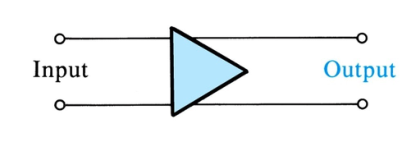
\includegraphics[scale=0.5]{images/ampli.png} \end{center}

\begin{itemize}
    \item Gain en tension :
    $$A_v = \frac{v_O}{v_I} \quad \left[\unit{\volt\per\volt}\right]$$
    \item Gain en courant :
    $$A_i = \frac{i_O}{i_I} \quad \left[\unit{\ampere\per\ampere}\right]$$
    \item Gain en puissance :
    $$A_p = A_v\cdot A_i \quad \left[\unit{\watt\per\watt}\right]$$
    \item Rendement :
    $$\eta = \frac{P_L}{P_{dc}} \times 100 \quad \left[\%\right]$$
    
    $P_L$ : Puissance sur la charge

    $P_{dc} = V_{CC}\cdot I_{CC} + V_{EE}\cdot I_{EE}$
\end{itemize}

Gain en dB : $20\cdot \log|A|$

\subsection{Amplificateur idéal}

\begin{center} 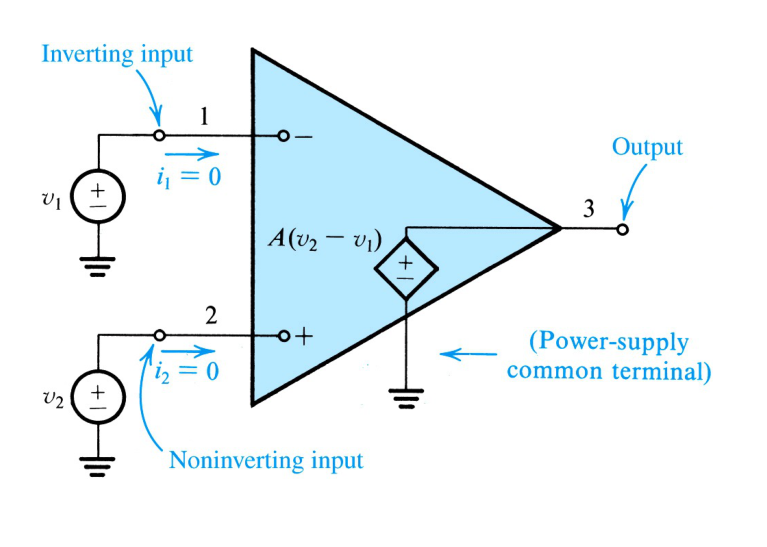
\includegraphics[scale=0.35]{images/ampli-ideal.png} \end{center}

\begin{itemize}
    \item Impédance d'entrée infinie
    \item Impédance de sortie nulle
    \item Gain de mode commun nul
    \item Gain en boucle ouverte (A) infini
    \item Bande passante (fréquence) infinie
\end{itemize}

\subsection{Réponse en fréquence en boucle ouverte}

$$\boxed{A(j\omega) = \frac{A_O}{1 + j\omega/\omega_b}}$$

GBW : $\omega_t = A_O \cdot \omega_b$  (fréquence à laquelle le gain vaut $1$)

\subsection{Boucle fermé : Inverting configuration}

Notation : $A$ pour l'amplificateur seul, et $G$ pour le montage

\begin{center} 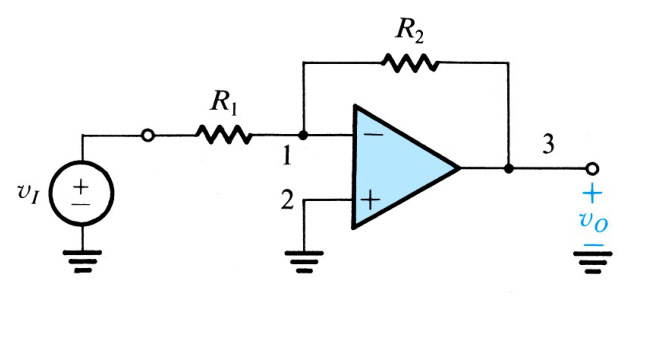
\includegraphics[scale=0.4]{images/inverting.png} \end{center}

$$G = -\frac{R_2}{R_1}$$


\subsubsection{Effet de la réponse en fréquence}

\begin{center} 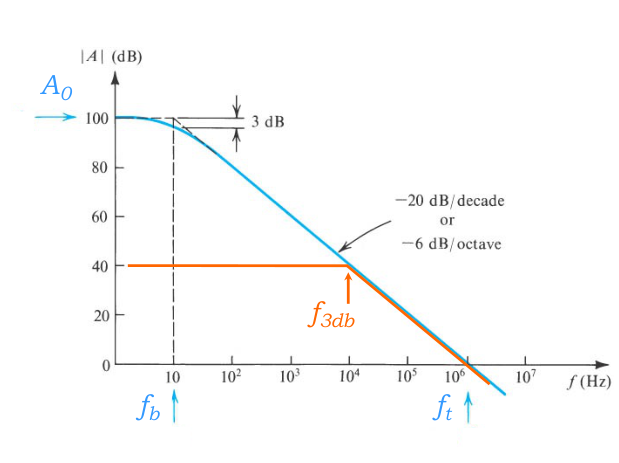
\includegraphics[scale=0.5]{images/ampli-ferme-freq.png} \end{center}

$$\frac{V_o(s)}{V_i(s)} \approx \frac{-R_2 / R_1}{1+\frac{s}{\omega_t/(1+R_2/R_1)}}$$

Pôle : $\omega_{3dB} = \omega_t / (1 + R_2/R_1)$

\subsection{Avec résistances interne}

\begin{center} 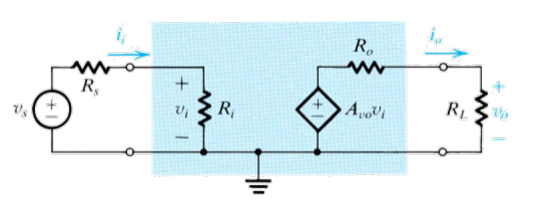
\includegraphics[scale=0.5]{images/quadripole.png} \end{center}

$$ \boxed{G_v = A_{vo} \frac{R_i}{R_i + R_s} \frac{R_L}{R_L + R_o}} $$

\subsection{Modèles de circuits pour amplificateurs}

\begin{center} 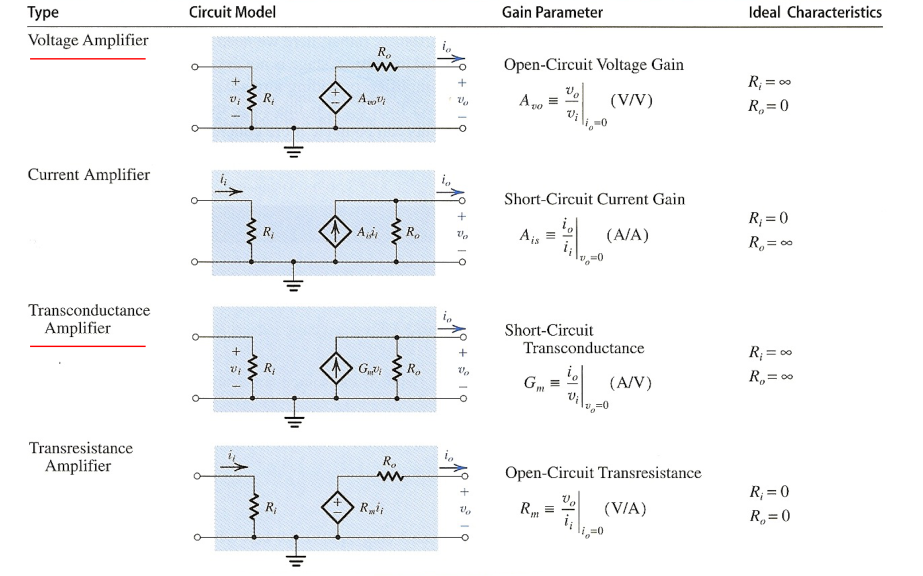
\includegraphics[scale=0.45]{images/model-circuits.png} \end{center}

\subsection{Amplificateurs avec étages en cascade}

\begin{center} 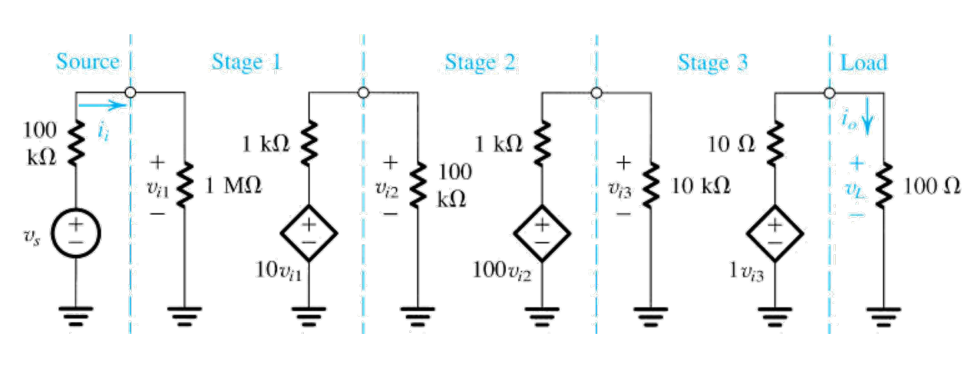
\includegraphics[scale=0.35]{images/ampli-cascade.png} \end{center}
$$R_s << R_{i,\text{étage }1} \qquad ; \qquad R_{o, \text{étage }i-1} << R_{i,\text{étage }i} \qquad ; \qquad R_{o,\text{étage }3 << R_L}$$
$$ \boxed{G_v = A_{vo} \frac{R_i}{R_i + R_s} \frac{R_L}{R_L + R_o}} $$


\break

\section{Diode}

\subsection{Diode idéale}

\begin{center} 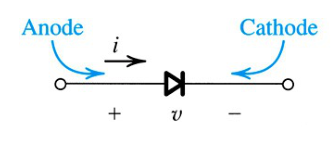
\includegraphics[scale=0.5]{images/diode.png} \end{center}

Tension négative : Bloquant

Tension positive : Passant

\subsubsection{Redresseur}

\begin{center} 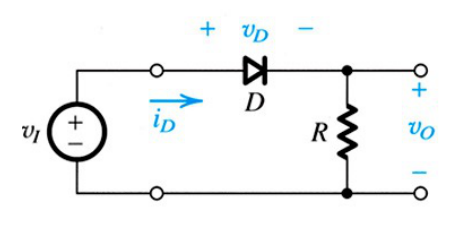
\includegraphics[scale=0.35]{images/redresseur.png} \end{center}

Fonctionne à basse fréquence, à haute fréquence, les effets capacitifs sont visible


\subsection{Diode réelle}

\begin{center} 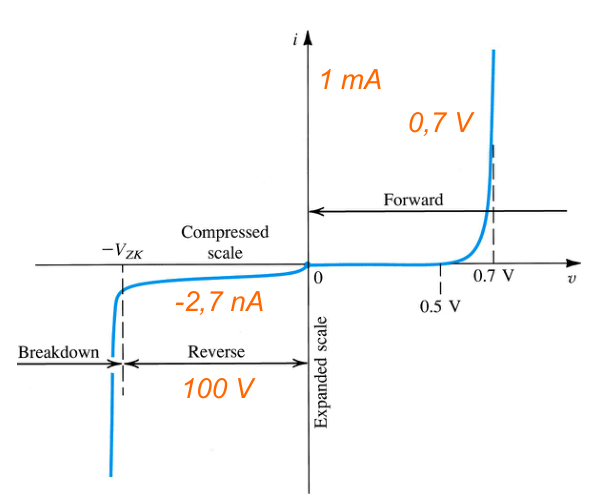
\includegraphics[scale=0.4]{images/diode-relle.png} \end{center}


\subsection{Modèle}

\begin{center} 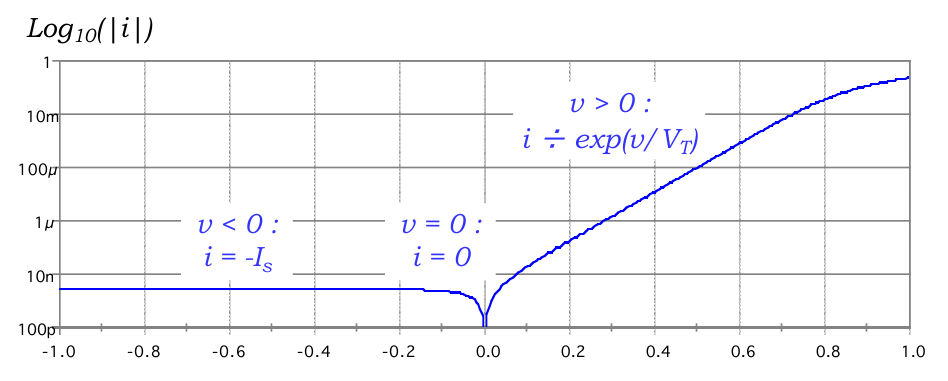
\includegraphics[scale=0.4]{images/modele-diode.png} \end{center}

$$ i = I_S \cdot \left(e^{v / (n \cdot V_T)} - 1\right) \quad \text{avec} \quad V_T = \frac{k \cdot T}{q} $$

$n$ : Constante empirique entre $1$ et $2$

$k$ : Constante de Boltzmann ($1.38 \; 10^{-23}$)

$T$ : Température en kelvins

$q$ : Charge électronique élémentaire ($1.6 \; 10^{-19}$)

$\Rightarrow V_T \approx 26 \unit{m\volt}$

\subsubsection{En sens passant}

\begin{center} 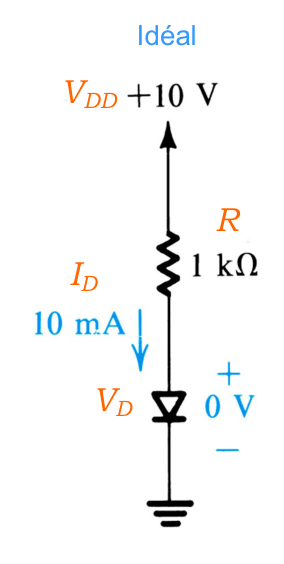
\includegraphics[scale=0.3]{images/model-sens-passant.png} \end{center}

$$I_D \approx I_s e^{V_D/V_T}$$
$$I_D = \frac{V_DD - V_D}{R}$$

On obtient $V_D \approx 0.7 \unit{\volt}$ et $I_D \approx 9.3 \unit{m\ampere}$


\subsubsection{Modèle petit-signal}

Cas de superposition d'un signal de polarisation (dc) et d'un signal alternatif (ac)

$$v_D(t) = V_D + v_d(t)$$
$$i_D(t) = I_D + i_d(t)$$

Concrètement, pour la partie AC, on peut remplacer la diode par une résistance $r_d$
$$r_d = \frac{1}{\left.\frac{\partial i_D}{\partial v_D}\right|_{i_D = I_D}} = \frac{(n) V_T}{I_D}$$

(Fonctionne bien jusqu'à des tensions alternatives d'environ $100 \unit{m\volt}$)


\break

\section{Mosfet}

NMOS : Flèche vers la capacité

PMOS : Flèche vers l'extérieur

\begin{comment}
\subsection{Régulateur LDO (Linear Drop Out)}

\begin{center} 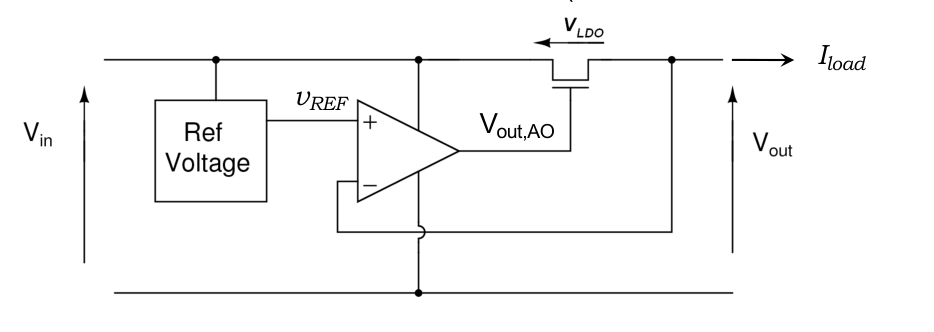
\includegraphics[scale=0.4]{images/regu-ldo.png} \end{center}
$$v_{OUT} = v_{IN} - R_{MOS}\cdot I_{load} \qquad \text{ssi} \qquad v_{IN} > v_{REF}$$
$$R_{MOS} = f(V_{out,AO}) \qquad \text{telle que} \qquad v_{OUT} = v_{REF}$$

<slide 3 avec simu spice>
\end{comment}

\subsection{Structure du transistor MOS}

\begin{center} 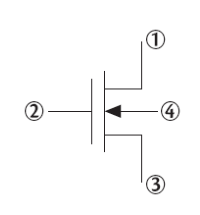
\includegraphics[scale=0.5]{images/mos.png} \end{center}

\begin{itemize}
    \item 1. Drain (D)
    \item 2. Grille (G)
    \item 3. Source (S)
    \item 4. Body ou Bulk
\end{itemize}

\begin{center} 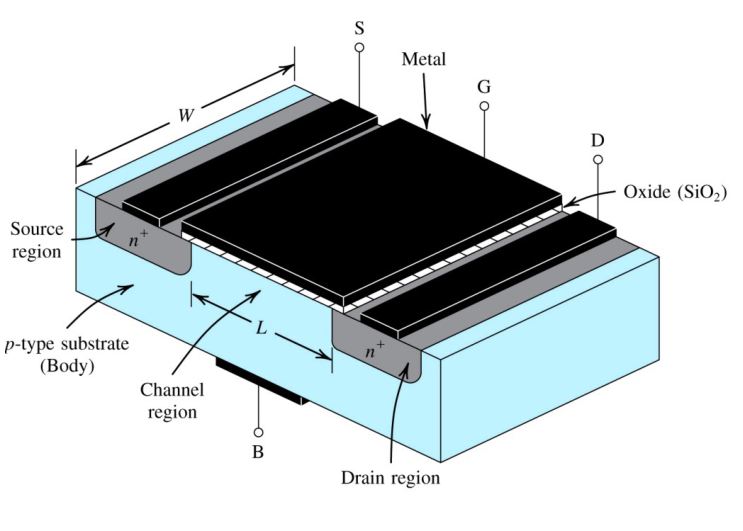
\includegraphics[scale=0.3]{images/struct-mos.png} \end{center}

\subsubsection{Technologie MOS complémentaire ou CMOS}

\begin{center} 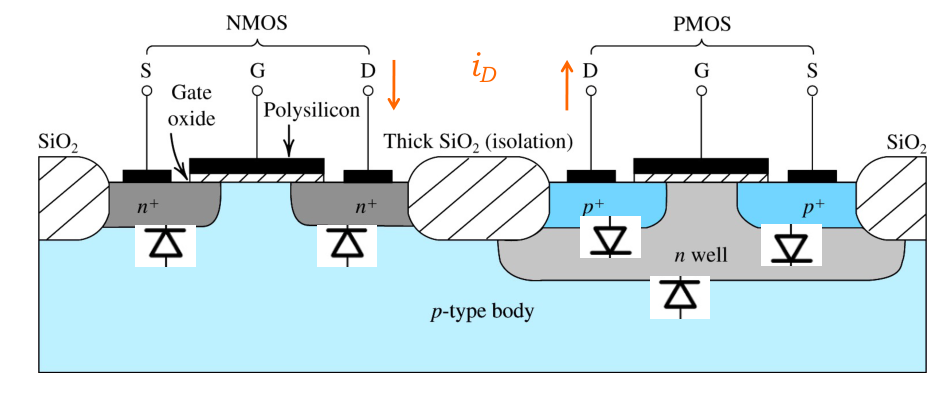
\includegraphics[scale=0.3]{images/nmos-pmos.png} \end{center}

Le drain et la source sont interchangable


\subsection{Caractéristiques Courant - Tensions}

Symbôles du NMOS :

\begin{center} 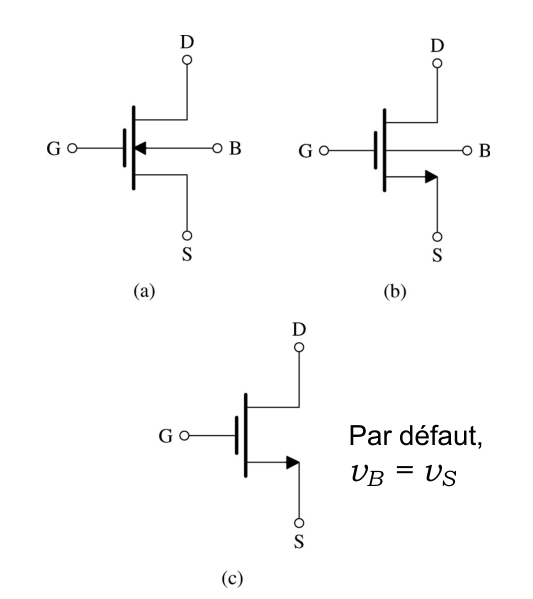
\includegraphics[scale=0.35]{images/symbol-nmos.png} \end{center}


\subsection{Régions de fonctionnement du NMOS}

\begin{center} 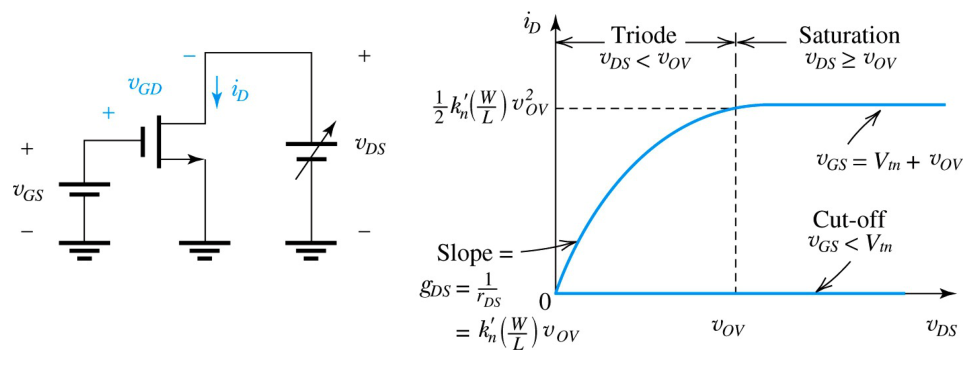
\includegraphics[scale=0.4]{images/mode-nmos.png} \end{center}

\begin{itemize}
    \item $v_{GS} < V_{tn}$ : $i_D \approx 0$ (régime \textbf{coupé} ou \textbf{cut-off})
    \item \textbf{Overdrive} $v_{OV} \triangleq v_{GS} - V_{tn} > 0$ : $i_D > 0$ (régime \textbf{passant} ou \textbf{turned-on})
    \begin{itemize}
        \item $v_{DS} < v_{OV}$ : $i_D (v_{DS}, v_{OV})$ (régime \textbf{triode})
        \item $v_{DS} \geq v_{OV}$ : $i_D (v_{OV})$ (régime \textbf{saturé})
    \end{itemize}
\end{itemize}

($V_{tn}$ est la tension seuil)


\subsection{Équations I-V}

\begin{center} 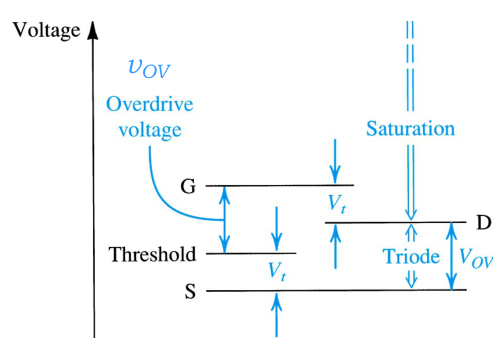
\includegraphics[scale=0.45]{images/nmos-eq.png} \end{center}

\textbf{Région de saturation} :

$$v_{DS} \geq v_{OV} \Leftrightarrow v_{GD} \leq V_{tn}$$
\begin{flalign*}
\rightarrow i_D &= \frac{1}{2} k_n' \frac{W}{L}(v_{GS} - V_{tn})^2\\
&= \frac{1}{2}k_n'\frac{W}{L} v_{OV}^2
\end{flalign*}

($k_n'$, $W$ et $L$ sont des paramètres du NMOS)

$k_n \text{ ou } \beta = k_n' \cdot W / L$

\medskip

\textbf{Région triode} :

$$ v_{DS} < v_{OV} \Leftrightarrow v_{GD} > V_{tn} $$
$$i_D = k_n' \frac{W}{L} \left[ v_{OV} - \frac{1}{2}v_{DS} \right] \cdot v_{DS} $$

si $v_{DS}$ faible :

$$i_D \approx k_n' \frac{W}{L} v_{OV} \cdot v_{DS}$$

\medskip

\textbf{En réalité} :

\begin{itemize}
    \item À $v_{DS}$ faible et $v_{GS}$ élevé, $i_D$ quasi-linéaire $\rightarrow$ résistance MOS
    \item En saturation, $i_D$ augmente légèrement avec $v_{DS}$ (effet Early ou 'modulation de longueur de canal')
\end{itemize}

$$\rightarrow \quad i_D = \frac{1}{2} k_n' \frac{W}{L} (v_{GS} - V_t)^2 (1 + \lambda v_{DS})$$

Tension d'Early : $V_A = 1/\lambda$

\begin{center} 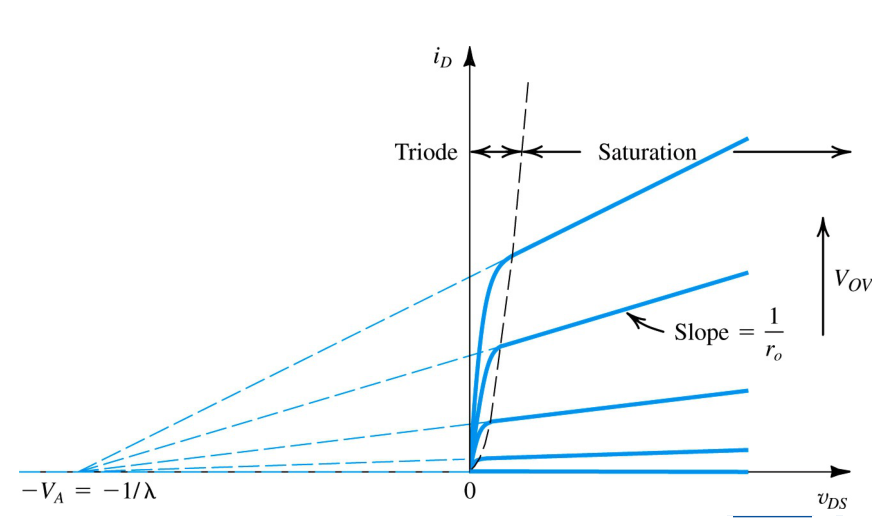
\includegraphics[scale=0.25]{images/early.png} \end{center}

%(Masse petit signal peut être 5V par exemple)


\subsection{Transistor PMOS}

\begin{center} 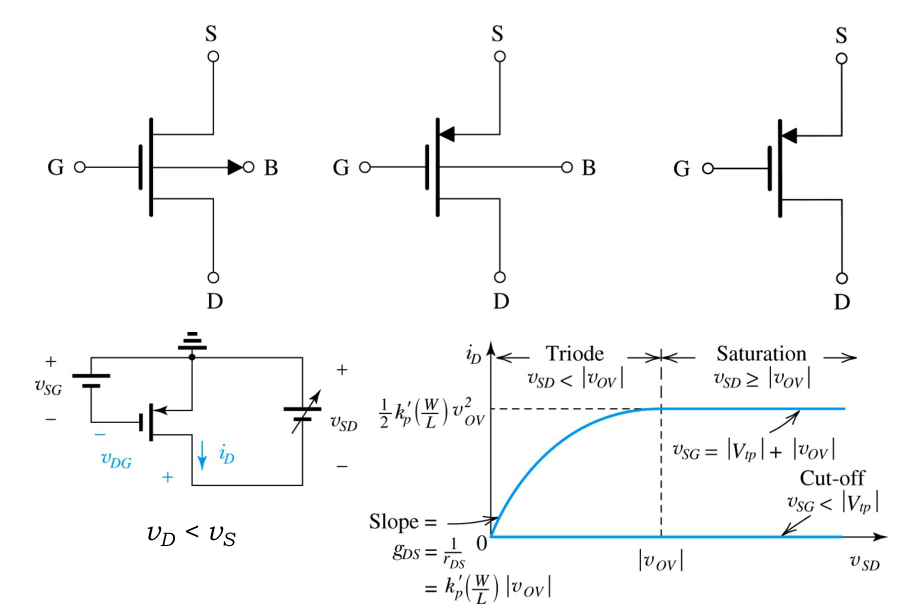
\includegraphics[scale=0.45]{images/pmos.png} \end{center}

\begin{center} 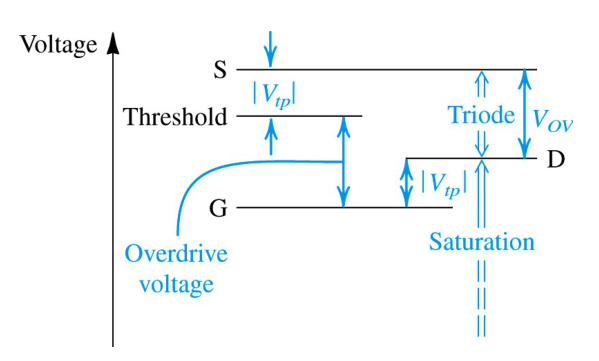
\includegraphics[scale=0.3]{images/pmos-iv.png} \end{center}

\textbf{Saturation Region} :

$$v_{SD} \geq |v_{OV}| \Leftrightarrow v_{DG} \leq |V_{tp}|$$

$$i_D = \frac{1}{2} k_p' \frac{W}{L}(v_{GS} - |V_{tp}|)^2 \cdot (1 + |\lambda_p|\cdot v_{SD})$$

\textbf{Triode Region} :

$$v_{SD} < |v_{OV}| \Leftrightarrow v_{DG} > |V_{tp}|$$

$$i_D = k_p' \frac{W}{L}\left[|v_{OV} - \frac{1}{2} v_{SD}\right] \cdot v_{SD}$$



\end{document}
